% \documentclass{standalone}
% \usepackage{currfile,hyperxmp}

% \input{../tikz_header.tex}

% \begin{document}

  
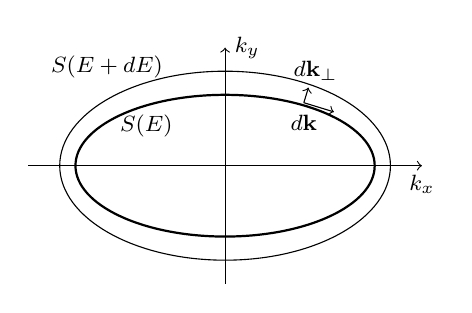
\begin{tikzpicture}[font=\footnotesize]

%\useasboundingbox (-1.3,-1.2) rectangle (11.2,4.7);
%	\draw (0,0) rectangle (5,4);

  
%\clip (-26mm,-16mm) rectangle  (26mm, 16mm);  
 
  
\draw[->] (-2.5,0) -- (2.5,0) node [below] {$k_x$};  
  \draw[->] (0,-1.5) -- (0,1.5) node [right] {$k_y$};  

\draw[thick] (0,0) ellipse (1.9cm and 0.9cm);
\draw[] (0,0) ellipse (2.1cm and 1.2cm);

\node at (-10mm, 5mm) {$S(E)$};
\node at (-15mm, 12.5mm) {$S(E + dE)$};


\draw[->] (10mm,8mm) -- node (a) {} ++ (73:2mm);
\draw[->] (10mm,8mm) -- ++ (-17:4mm);

\node at (11.5mm, 12mm) {$d\mathbf{k}_\perp$};
\node at (10mm, 5.5mm) {$d\mathbf{k}$};



  
  \end{tikzpicture}


%\end{document}
